\documentclass[aspectratio=169]{beamer}

\usepackage{amsmath}
\usepackage{amssymb}
\usepackage{mathtools}
\usepackage{wrapfig}
\usepackage{pgfplots}
\usepackage{tikz}
\usetikzlibrary{arrows.meta,positioning,shapes.geometric,shapes.misc}

\title{Solving Constrained Piecewise Linear Optimization Problems}
\author{Michael van Straten}
\date{\today}
\institute{Humboldt-Universität zu Berlin}

\DeclarePairedDelimiter{\set}{\lbrace}{\rbrace}
\DeclarePairedDelimiterXPP{\abs}[1]
    {}
    {\lvert}{\rvert}
    {}
    {\ifblank{#1}{\anyarg}{#1}}
\DeclarePairedDelimiter{\parens}{\lparen}{\rparen}

\newcommand{\field}[1]{\mathbb{#1}}
\newcommand{\reals}{\field{R}}
\newcommand{\sign}{\operatorname{sign}}
\newcommand{\sgn}{\operatorname{sgn}}

\begin{document}

\begin{frame}
    \titlepage

    \note{
        In this talk I will be presenting an algorithm for solving
        finite-dimensional optimization problems with a piecewise linear
        objective function and piecewise linear constraints. This algorithm
        was developed by Dr. Timo Kreimeier under the supervision of Prof. Dr.
        Andrea Walther and Prof. Dr. Andreas Griewank, who was significantly
        involved in the initial ideas of this work.
    }
\end{frame}

\begin{frame}{Motivation}
    \begin{itemize}[<+->]
        \item A function $f \colon \reals^n \to \reals$ is \textbf{PL}
              (Piecewise Linear) \(\iff\) there exists a finite set of affine
              linear functions $f_{i \in \set{1, \dots, k}}(x)$ such that
              \[
                  f(x) \in \set{f_1(x), f_2(x), \dots, f_k(x)}
                  \forall x \in \reals^n.
              \]
        \item<2-> Piecewise composition creates non-differentiable points
        \item<3-> Classical optimization methods (SQP, Newton, trust-region)
              require gradients
        \item<4-> Algorithmic differentiation tools exist for smooth functions
        \item<5-> Nonsmooth functions lack derivative information at kinks
        \item<6-> Applications: train timetabling, neural networks (ReLU),
              inventory problems
        \item<7-> Mixed-integer optimization problems are NP-hard
    \end{itemize}

    \note<1>{
        Definition of piecewise linear functions: they can be represented as a
        finite set of affine linear functions.
    }
    \note<2>{
        The piecewise composition leads to points in the domain where the
        function is no longer differentiable, making derivative-based
        optimization algorithms difficult to apply.
    }
    \note<3>{
        In smooth optimization, classical approaches like trust-region methods,
        sequential quadratic programming (SQP) or Newton's methods require
        gradients of the original problem. These methods rely on Taylor
        expansion to produce approximations with local errors of appropriate
        order.
    }
    \note<4>{
        For smooth functions, gradients exist theoretically and can be computed
        numerically using algorithmic differentiation (AD). Examples include
        ADOL-C, TAPENADE, CoDiPack for C/C++, and ADiMAT for Matlab.
    }
    \note<5>{
        For nonsmooth functions, derivative information is not available at
        every point, making Taylor expansion impossible. Andreas Griewank
        addressed this in 2013 with piecewise linearization for Lipschitz
        continuous functions. According to Rademacher's theorem, Lipschitz
        continuous functions are differentiable almost everywhere, and a
        second-order approximation property can be shown for this approach.
    }
    \note<6>{
        Applications include train timetabling, shallow training of neural
        networks with ReLU activation, inventory problems, and mixed-integer
        optimization problems. The second-order approximation property
        motivates using such algorithms as inner solvers for general nonsmooth
        problem algorithms like SALMIN.
    }
    \note<7>{
        Mixed-integer optimization problems are NP-hard, including piecewise
        linear optimization problems even when using exact penalty methods.
        These arise in applications like gas network optimization through
        mixed-integer linear relaxations.
    }
\end{frame}

\section{The Active Signature Method}

\begin{frame}{Overview}
    \begin{itemize}[<+(1)->]
        \item Each piecewise linear function can be represented as a
              combination of \(\min\) and \(\max\) functions
        \item \(\max\) and \(\min\) functions can be represented using
              \(\abs{\cdot}\):
              \[
                  \min(x, y) = \frac{1}{2}(x + y - \abs{x - y})
                  \text{ and }
                  \max(x, y) = \frac{1}{2}(x + y + \abs{x - y})
              \]
        \item Active Signature Method (ASM) solves unconstrained piecewise
              linear optimization problems
        \item Transform objective function \(f \colon \reals^n \to \reals\) to
              \(\tilde{f} \colon \reals^n \times \reals^s \to \reals\)
        \item This transformed version is called Abs-Linear Forms
    \end{itemize}

    \note<1>{
        Stefan Scholtes showed in ``Introduction to Piecewise Linear
        Optimization'' Proposition 2.2.2 that each piecewise linear function
        can be represented as a combination of \(\min\) and \(\max\) functions.
    }
    \note<2>{
        This representation using absolute values is fundamental to the method
        we will discuss.
    }
    \note<3>{
        For unconstrained piecewise linear optimization problems, Andrea
        Walther and Andreas Griewank already presented a solution algorithm
        called the Active Signature Method (ASM) in 2019.
    }
    \note<4>{
        The basic idea is to transform an objective function
        \(f \colon \reals^n \to \reals\) to a function
        \(\tilde{f} \colon \reals^n \times \reals^s \to \reals\) so that
        constraining the second argument results in \(\tilde{f}\) being linear.
    }
    \note<5>{
        We will discuss this transformation, called Abs-Linear Forms, in detail
        later.
    }
\end{frame}

\begin{frame}{Abs Linear Forms}
    A continuous piecewise linear function
    \(f \colon \reals^n \to \reals\) is said to be in \textbf{Abs-Linear
        Form} if \(y = f(x)\) is given by
    \begin{align*}
        y & = a^T x + b^T z                     \\
        z & = c + Z x + M z + L \abs{z} \tag{*}
    \end{align*}
    with \(x \in \reals^n\) the argument vector, \(z \in \reals^s\),
    \(a \in \reals^n\), \(b, c \in \reals^s\), \(Z \in \reals^{s \times n}\),
    \(L, M \in \reals^{s \times s}\). Where the last two matrices are strictly
    lower triangular.

    \begin{itemize}[<+(1)->]
        \item \(z \in \reals^s\) is the switching vector
        \item Forward substitution solves (*) for \(z\) in terms of \(x\)
        \item AD software computes Abs-Linear forms automatically
    \end{itemize}

    \note<2>{
        The vector \(z \in \reals^s\) is called the switching vector with
        (*) denoting the switching equation.
    }
    \note<3>{
        Since \(M\) and \(L\) are strictly lower triangular, the equation
        (*) can be solved for \(z\) in terms of \(x\) using forward
        substitution.
    }
    \note<4>{
        AD software like ADOL-C, which was developed by Prof. Dr. Andrea
        Walther and Prof. Dr. Andreas Griewank, can compute the Abs-Linear
        form for any PL function.
    }
\end{frame}

\begin{frame}{Example Abs-Linear Form}
    \begin{wrapfigure}{r}{0.4\textwidth}
        \centering
        \onslide<1->{
            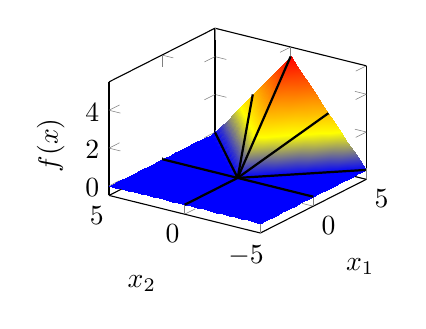
\begin{tikzpicture}
                \begin{axis}[
                        width=0.4\textwidth,
                        xlabel=$x_1$,
                        ylabel=$x_2$,
                        zlabel={$f(x)$},
                        xmin=-5, xmax=5,
                        ymin=-5, ymax=5,
                        xtick={0,5}, ytick={-5,0,5}, view={305}{30}
                    ]
                    \addplot3[ surf, shader=interp ] {max(0,x-abs(y))};

                    \draw [black, thick] (axis cs:0,0,0) -- (axis cs:5,5,0);
                    \draw [black, thick] (axis cs:0,0,0) -- (axis cs:5,-5,0);
                    \draw [black, thick] (axis cs:0,0,0) -- (axis cs:5,0,5);
                    \draw [black, thick] (axis cs:0,-5,0) -- (axis cs:0,5,0);
                    \draw [black, thick] (axis cs:0,0,0) -- (axis cs:-5,0,0);
                    \draw [black, thick] (axis cs:0,0,0) --
                    (axis cs:5,2.5,2.5);
                    \draw [black, thick] (axis cs:0,0,0) --
                    (axis cs:5,-2.5,2.5);
                \end{axis}
            \end{tikzpicture}
        }
    \end{wrapfigure}

    \onslide<1->{
        Consider the function \(f(x) : \reals^2 \to \reals\)
        \begin{align*}
            \onslide<1-> {f(x) & = \max\{0, x_1 - |x_2|\} \\}
            \onslide<2-> {     & = \frac{1}{2} (x_1 − \abs{x_2} +
                \abs{x_1 - \abs{x_2}}).}
        \end{align*}
    }

    \onslide<3->{
        The Abs-Linear form is given by
        \[
            y = \begin{bmatrix}
                \frac{1}{2} & 0
            \end{bmatrix}
            \begin{bmatrix}
                x_1 \\ x_2
            \end{bmatrix}
            + \begin{bmatrix}
                0 & 0 & 1
            \end{bmatrix}
            \begin{bmatrix}
                z_1 \\ z_2 \\ z_3
            \end{bmatrix}, \text{ and}
        \]
    }
    \onslide<4->{
        \[
            z = \begin{bmatrix}
                x_2 \\ x_1 - \abs{z_1} \\ -\frac{1}{2}\abs{z_1} + \abs{x_2}
            \end{bmatrix} =
            0_{\reals^3}
            + \begin{bmatrix}
                0 & 1 \\ 1 & 0 \\ 0 & 0
            \end{bmatrix}
            \begin{bmatrix}
                x_1 \\ x_2
            \end{bmatrix}
            +
            0_{\reals^{3 \times 3}}
            \begin{bmatrix}
                x_1 \\ x_2
            \end{bmatrix}
            +
            0_{\reals^{3 \times 3}}
            \begin{bmatrix}
                z_1 \\ z_2 \\ z_3
            \end{bmatrix}
            +
            \begin{bmatrix}
                0 & 0 & 0 \\ -1 & 0 & 0 \\ -\frac{1}{2} & -\frac{1}{2} & 0
            \end{bmatrix}
            \begin{bmatrix}
                \abs{z_1} \\ \abs{z_2} \\ \abs{z_3}
            \end{bmatrix}
        \]
    }

    \note{
        Because of its shape, this function will be referred to as
        Hill-function in the following. Note that this is a nonsmooth and
        nonconvex function, which in particular is already piecewise linear.
        The points where the function is not differentiable in the classical
        sense are marked by dark blue lines. The idea here is to use \(z\) to
        encode the inner absolute values of \(f\).
    }
\end{frame}

\begin{frame}{Characterizing non-smoothness using \(z\)}
    \begin{wrapfigure}{r}{0.5\textwidth}
        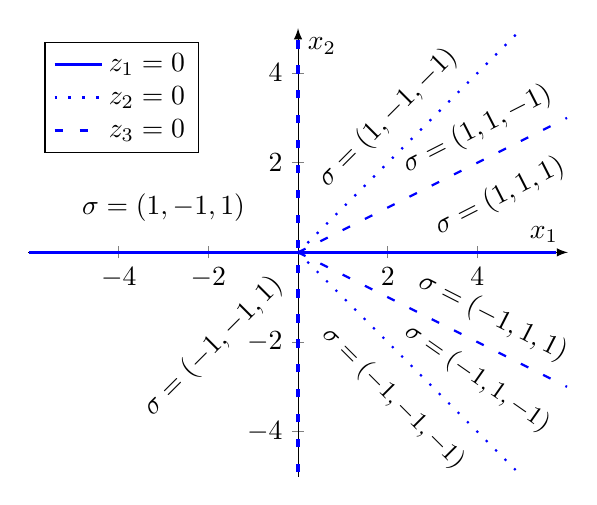
\begin{tikzpicture}
            \begin{axis}[
                    axis equal,
                    axis lines=middle,
                    axis line style={-latex},
                    xlabel=$x_1$,
                    ylabel=$x_2$,
                    xmin=-5, xmax=5,
                    ymin=-5, ymax=5,
                    xtick={-4,-2,0,2,4},
                    ytick={-4,-2,0,2,4},
                    legend pos=north west
                ]

                % kink due to z1
                \draw [blue, very thick] (axis cs:-6,0) -- (axis cs:5.75,0);
                \addlegendimage{line width=1pt,color=blue}
                \addlegendentry{$z_1=0$}

                % kinks due to z2
                \draw [blue, thick, loosely dotted] (axis cs:0,0) --
                (axis cs:5,5);
                \draw [blue, thick, loosely dotted] (axis cs:0,0) --
                (axis cs:5,-5);
                \addlegendimage{line width=1pt,color=blue,style=loosely dotted}
                \addlegendentry{$z_2=0$}

                % kinks due to z3
                \draw [blue, very thick, loosely dashed] (axis cs:0,-4.9) --
                (axis cs:0,4.75);
                \draw [blue, thick, loosely dashed] (axis cs:0,0) --
                (axis cs:6,3);
                \draw [blue, thick, loosely dashed] (axis cs:0,0) --
                (axis cs:6,-3);
                \addlegendimage{line width=1pt,color=blue,style=loosely dashed}
                \addlegendentry{$z_3=0$}

                \node[rotate=0] at (axis cs: -3,1) {$\sigma=\parens{1,-1,1}$};
                \node[rotate=45] at (axis cs: 2,3) {$\sigma=\parens{1,-1,-1}$};
                \node[rotate=27] at (axis cs: 4,2.75) {$\sigma=\parens{1,1,-1}$};
                \node[rotate=27] at (axis cs: 4.5,1.25) {$\sigma=\parens{1,1,1}$};
                \node[rotate=-27] at (axis cs: 4.35,-1.45)
                {$\sigma=(-1,1,1)$};
                \node[rotate=-35] at (axis cs: 4,-2.8)
                {\small $\sigma=(-1,1,-1)$};
                \node[rotate=-45] at (axis cs: 2.125,-3.25)
                {\small $\sigma=(-1,-1,-1)$};
                \node[rotate=45] at (axis cs: -1.9,-2.1)
                {$\sigma=(-1,-1,1)$};
            \end{axis}
        \end{tikzpicture}
    \end{wrapfigure}
    Let signature vector of \(z \in \reals^s\) be
    \[
        \sgn(z)_i = (\sign(z_i)) \in \{-1, 0, 1\}
    \]
    Looking at our hill function example from the previous slide:

    \begin{itemize}[<+(1)->]
        \item Signature vector \(\sgn(z)\) changes across input domain
        \item Each sign flip corresponds to different polyhedron
        \item Boundares \(\sgn(z)_i = 0\) encodes the potential non-smooth
              points of the system.
        \item Regions where \(\sgn(z)\) is fixed represent are called signature
              domain.
    \end{itemize}

    \note<1>{
        The signature vector \(\sgn(z)\) is a vector of length \(s\) where
        each element \(\sgn(z)_i\) is the sign of the corresponding element
        \(z_i\) in \(z\).
    }

    \note<2>{
        With our example hill function, we can observe how the signature vector
        \(\sgn(z)\) changes across different regions of the input domain,
        creating distinct behavioral patterns.
    }

    \note<3>{
        We note that each sign flip in the signature vector corresponds to a
        different polyhedron in the input space, effectively partitioning the
        domain into regions with consistent linear behavior.
    }

    \note<4>{
        Since our switching equation is linear when we cross from one
        polyhedron to another, the signature vector has to be 0 in one
        component at the boundary between two polyhedra, representing the
        transition point. These points encode the non-smooth behavior of the
        system.
    }

    \note<5>{
        The regions where the signature vector \(\sgn(z)\) is fixed are called
        signature domains. These domains represent regions of the input space
        where the system exhibits consistent linear behavior.
    }
\end{frame}

\begin{frame}{Reduction to a quadratic optimization problem with linear
        constraints}
    Let us now fix the signature vector \(\sigma := \sgn(z)\) to a specific
    value within a signature domain.

    Therefore, consider for each fixed \(\sigma \in \{-1, 0, 1\}^s\) the
    optimization problem
    \begin{align}
        \min_{x \in \reals^n, z \in \reals^s} \quad & a^T x + b^T z
        \onslide<2->{+ \frac{1}{2}x^TQx}                                          \\
        \text{s.t.} \quad                           & z = c + Zx + Mz + L\Sigma z \\
                                                    & 0 = (I_s - |\Sigma|)z       \\
                                                    & 0 \leq \Sigma z
    \end{align}
    where \(\Sigma = \text{diag}(\sigma)\) and \(|\Sigma| = \text{diag}(|\sigma|)\).

    \begin{itemize}[<+(1)->]
        \item To bound the objective function from below we introduce a
              quadratic penaltry term using a positive definite matrix \(Q \in
              \reals^{n \times n}\)
    \end{itemize}
\end{frame}

\begin{frame}{Computing a decent direction}
    To determine a descent direction, KKT-theory is applied to arive at the
    following system of linear equations
    \[
        \begin{bmatrix}
            Q          & 0            & -\tilde{Z}^{\top} \\
            0          & 0            & \abs{\Sigma}      \\
            -\tilde{Z} & \abs{\Sigma} & 0
        \end{bmatrix}
        \begin{bmatrix}
            x \\
            z \\
            \lambda
        \end{bmatrix}
        =
        \begin{bmatrix}
            -a              \\
            -\abs{\Sigma} b \\
            \tilde{c}
        \end{bmatrix},
    \]
    where
    \[
        \tilde{Z} := (I_s - M - L\Sigma)^{-1} Z \quad \text{and} \quad
        \tilde{c} := (I_s - M - L\Sigma)^{-1} c.
    \]
\end{frame}

\begin{frame}{Computing a step size}
    After computing a search direction $\Delta x$ we choose a step length
    $\beta>0$ such that the next iterate
    \[
        x^{+} = x + \beta\,\Delta x \quad (\,= (1-\beta)x + \beta \hat{x}\,)
    \]
    remains inside the current signature domain $\mathcal P_{\sigma}$.

    \medskip
    \textbf{1.  Candidate step size $\beta^{z}$.}  For the switching vector
    $z\in\mathbb R^{s}$ and its update $\hat z = z + \beta\,\Delta z$ we
    detect the first component that would change its sign:
    \[
        \beta^{z}=\inf_{1\le i \le s} \Bigl\{\;\beta_i^{z}=\frac{-z_i}{\hat z_i-z_i}
        \;\Bigm|\;(\hat z_i-z_i)\,\sigma_i<0\Bigr\}\in[0,\infty] .  \tag{3.32}
    \]

    \begin{itemize}[<+(1)->]
        \item If $\beta^{z}=\infty$ a \emph{full} step can be taken
              $(\beta=1)$.
        \item Otherwise $\beta^{z}\le 1$ hits the blocking kink~$j^{z}$ and the
              signature must be updated.
    \end{itemize}

    \medskip
    \textbf{2.  Final step size.}  We bound the step to stay in
    $\overline{\mathcal P}_{\sigma}$:
    \[
        \boxed{\;\beta = \min\{\beta^{z},\,1\}\;} \quad\text{and}\quad
        x^{+}=x+\beta\,\Delta x. \tag{3.33}
    \]

    A point with $\beta=1$ is called \emph{signature stationary} because the
    iterate does not leave the current domain.
\end{frame}

\begin{frame}{Checking the optimality}
    Even when a point is \emph{signature stationary}, we must verify if it's optimal for (ALOP).

    \medskip
    Replace $\Sigma$ by $\Sigma+\Gamma$ where $\Gamma$ contains relaxed components $\gamma\succ 0$.
    The complementarity condition becomes
    \[
        0 \;\le\; \mu^{\top}|\Gamma| \;=
        b^{\top}\Gamma + \lambda^{\top}\Gamma - \lambda^{\top}\tilde{L}|\Gamma|
        \quad (\approx 0).
    \]

    The optimality test fails if there exists an index $k$ with
    \[
        0 > -\bigl(b^{\top}+\lambda^{\top}\bigr)\,e_k - \lambda^{\top}\tilde{L}e_k
        \quad\text{and}\quad \sigma_k = 0.\tag{3.34}
    \]

    \begin{itemize}[<+(1)->]
        \item Choose index $k$ with largest violation and update $\sigma_k^{+}
              := -\operatorname{sgn}\bigl(b_k+\lambda_k\bigr)$
        \item Release the corresponding absolute value (relax the kink)
        \item Continue on neighbouring polyhedron $\mathcal{P}_{\sigma^{+}}$
    \end{itemize}
\end{frame}

\begin{frame}{Overall algorithm flow}
    \centering
    \begin{figure}
        \includegraphics[width=0.6\textwidth]{assets/asm.png}
    \end{figure}
\end{frame}

\begin{frame}{ASM for Hill-Example}
    \begin{figure}
        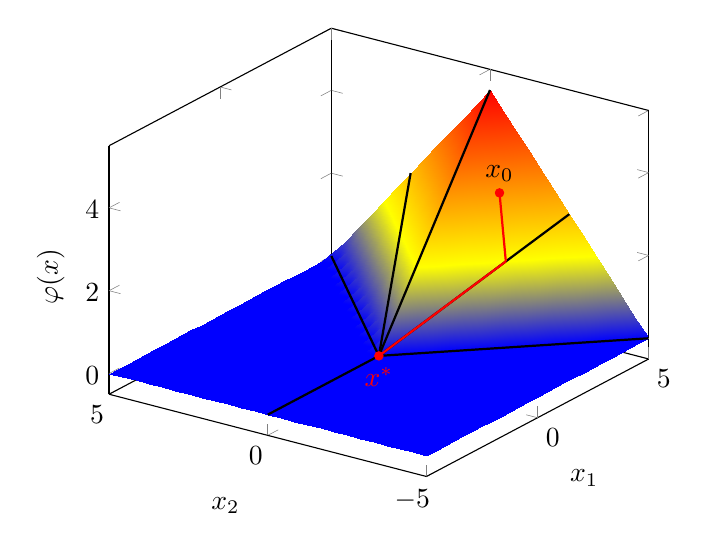
\begin{tikzpicture}
            \begin{axis}[
                    xlabel=$x_1$,
                    ylabel=$x_2$,
                    zlabel={$\varphi(x)$},
                    xmin=-5, xmax=5,
                    ymin=-5, ymax=5,
                    xtick={0,5},
                    ytick={-5,0,5},
                    view={305}{30}
                ]
                \addplot3[
                    surf,
                    shader=interp
                ] {max(0,x-abs(y))};

                \draw [black, thick] (axis cs:0,0,0) -- (axis cs:5,5,0);
                \draw [black, thick] (axis cs:0,0,0) -- (axis cs:5,-5,0);
                \draw [black, thick] (axis cs:0,0,0) -- (axis cs:-5,0,0);
                \draw [black, thick] (axis cs:0,0,0) -- (axis cs:5,0,5);
                \draw [black, thick] (axis cs:0,0,0) -- (axis cs:5,2.5,2.5);
                \draw [black, thick] (axis cs:0,0,0) -- (axis cs:5,-2.5,2.5);

                \node[label={[label distance=-3pt]90:$x_0$},mark size=1.5pt,
                    color=red] at (axis cs:4,-1,3) {\pgfuseplotmark{*}};

                \draw<2-> [red, thick] (axis cs:4,-1,3) --
                (axis cs:3.33311,-1.66656,1.66656);

                \draw<3-> [red, thick] (axis cs:3.33311,-1.66656,1.66656) --
                (axis cs:0,0,0);

                \node<4->[label={[label distance=-3pt,color=red]270:$x^*$},
                    mark size=1.5pt,color=red] at (axis cs:0,0,0)
                { \pgfuseplotmark{*} };
            \end{axis}
        \end{tikzpicture}
    \end{figure}
\end{frame}

\section{My work on CASM's implementation}

\begin{frame}{Background and Initial State}
    \begin{itemize}[<+->]
        \item Joined Prof. Dr. Walther's team to help publish CASM software
              package
        \item CASM C++ implementation originally by Dr. Sabrina Fiege, extended
              by Adrian Schmidt
        \item Codebase was a combination of C++ and MATLAB implementations in
              poor condition
        \item Main task: refactor codebase for software package publication
    \end{itemize}

    \note<1>{
        I joined the team last semester specifically to help with the
        publication of a software package for the Constrained Active Signature
        Method (CASM).
    }
    \note<2>{
        The original CASM C++ implementation was written by Dr. Sabrina Fiege
        and later extended and documented by Adrian Schmidt.
    }
    \note<3>{
        The codebase at this point was a combination of two different
        implementations - one in C++ and one in MATLAB - and was not in the
        best shape for publication.
    }
    \note<4>{
        My primary tasks were to refactor the codebase to bring it to a state
        where it can be used as a software package and published.
    }
\end{frame}

\begin{frame}{Repository Optimization}
    \begin{itemize}[<+->]
        \item Started by splitting codebase into separate parts with Adrian
        \item Optimized GitHub repository for clone speed
        \item Original repo contained many unnecessary files (400MB+)
        \item Used git filter-repo and Git LFS to reduce size to under 1MB
        \item Benefits: faster downloads and no exposure of unnecessary files
              (logs, binaries, etc.)
    \end{itemize}

    \note<1>{
        Adrian and I started by splitting the codebase into its separate parts
        to better organize the project structure.
    }
    \note<2>{
        I then optimized the GitHub repository for clone speed since the
        original repo contained a lot of unnecessary files.
    }
    \note<3>{
        The original repository was over 400MB in size due to various
        unnecessary files.
    }
    \note<4>{
        A git filter-repo job and moving files to Git Large File Storage (LFS)
        reduced the repo size from over 400MB to under 1MB.
    }
    \note<5>{
        This optimization is relevant for publishing because you want to be
        able to download the codebase quickly and not expose any unnecessary
        files to the public.
    }
\end{frame}

\begin{frame}{Bug Discovery and Fixes}
    \begin{itemize}[<+->]
        \item Started working with existing test suite
        \item Discovered bugs in ADOL-C library:
              \begin{itemize}
                  \item Heap Buffer Overflow due to signature buffer reuse
                  \item Container overflow and double free in
                        tape\_handling.cpp:588
              \end{itemize}
        \item These bugs were causing test failures in CASM test suite
        \item All identified bugs were fixed
    \end{itemize}

    \note<1>{
        I then started to try to run the already existing test suite which led
        me to discover some bugs in ADOL-C.
    }
    \note<2>{
        The main issues were a Heap Buffer Overflow due to reuse of a
        signatures buffer which contained the switching variables and which was
        not reallocated when the number of variables changed.
    }
    \note<3>{
        There was also another container-overflow and double free in cleanUp
        tape_handling.cpp:588.
    }
    \note<4>{
        These bugs were causing test failures in the CASM test suite and were
        fixed.
    }
\end{frame}

\begin{frame}{C++23 Modernization}
    \begin{itemize}[<+->]
        \item Refactored codebase to use new C++23 features
        \item Original code had some issues:
              \begin{itemize}
                  \item Matrix-vector multiplication implemented as for loops
                  \item Memory allocations using malloc and delete
              \end{itemize}
        \item Set up proper dependency management:
              \begin{itemize}
                  \item Git submodules
                  \item Meson build system
                  \item Nix for reproducible builds
              \end{itemize}
    \end{itemize}

    \note<1>{
        I've then started to refactor the codebase to make use of the new C++23
        features.
    }
    \note<2>{
        Since many routines, like matrix-vector multiplication, were implemented
        as for loops and allocations were mainly done using malloc and delete.
    }
    \note<3>{
        We also set up proper dependency management using git submodules and
        meson as well as nix for reproducible builds.
    }
\end{frame}

\begin{frame}{Eigen Library Integration}
    \begin{itemize}[<+->]
        \item Decided to refactor using popular Eigen library
        \item Significant code reduction: from 3000 to 600 lines
        \item Memory management improvements:
              \begin{itemize}
                  \item Automatic memory allocation using smart pointers
                  \item Reduced risk of memory leaks
                  \item Fewer bugs related to manual memory management
              \end{itemize}
        \item Expected performance improvements:
              \begin{itemize}
                  \item Advanced optimizations like vectorization
                  \item Offloading to dedicated libraries like OpenBLAS
              \end{itemize}
    \end{itemize}

    \note<1>{
        Since there was already a lot of code changing, I decided to refactor
        using the popular Eigen library.
    }
    \note<2>{
        I was able to bring down the number of lines of code from 3000 to 600.
    }
    \note<3>{
        Most memory allocations are now managed automatically using smart
        pointers which reduces the risk of memory leaks and other bugs related
        to manual memory management.
    }
    \note<4>{
        I also expect the performance to improve significantly since Eigen can
        do advanced optimizations like vectorization and offloading to
        dedicated libraries like OpenBLAS.
    }
\end{frame}

\begin{frame}[fragile]{Code Comparison: Before vs After}
    \begin{columns}[T]
        \begin{column}{0.48\textwidth}
            \begin{block}{}
                \tiny
                \begin{verbatim}
void casm::signature_vec(int dim, double *vec, short *signature,
                         const double eps)
{
    for (int i = 0; i < dim; i++)
    {
        if (fabs(vec[i]) < eps) {
            signature[i] = 0;
            vec[i] = 0; // Match 'signature' and 'vec':
                        // Set z=0 if kink is identified as active
        } else {
            signature[i] = (vec[i] >= eps) ? 1 : -1;
        }
    }
}
                \end{verbatim}
            \end{block}
        \end{column}

        \begin{column}{0.48\textwidth}
            \begin{block}{}
                \tiny
                \begin{verbatim}
inline auto SignatureVector(const Eigen::VectorXd &vec,
                           double eps = 1.0e-12) {
    return (vec.array().abs() < eps).select(0, vec.array().sign());
}
                \end{verbatim}
            \end{block}
        \end{column}
    \end{columns}
\end{frame}

\begin{frame}[fragile]{Code Comparison: Before vs After}
    \begin{columns}[T]
        \begin{column}{0.48\textwidth}
            \begin{block}{}
                \tiny
                \begin{verbatim}
void casm::EvaluateAbsLinearEqSystemAbsoluteValue(
    int dim_result, int n, int s, double *x, double *z, double *c,
    double **A, double **B, double **C, double *result)
{
    double *z_abs;
    double *Ax, Bz_i, Cz_abs_i;

    z_abs = (double *)calloc(s, sizeof(double));
    Ax = (double *)calloc(dim_result, sizeof(double));

    set_vec2const(dim_result, result, 0.0);

    for (int i = 0; i < s; i++)
        z_abs[i] = fabs(z[i]);

    MultiplyMatrixVector(dim_result, n, A, x, Ax);
    for (int i = 0; i < dim_result; i++)
    {
        Bz_i = ScalarProduct(s, B[i], z);
        Cz_abs_i = ScalarProduct(s, C[i], z_abs);
        result[i] = c[i] + Ax[i] + Bz_i + Cz_abs_i;

        if (z == result)
            z_abs[i] = fabs(z[i]);
    }

    free(z_abs);
    free(Ax);
}
                \end{verbatim}
            \end{block}
        \end{column}

        \begin{column}{0.48\textwidth}
            \begin{block}{}
                \tiny
                \begin{verbatim}
template <typename Derived>
Eigen::Matrix<double, s, 1> EvalSwitchingVector(
    const Eigen::MatrixBase<Derived> &x) const {
  // We'll compute c + Z * x once
  Eigen::VectorXd c_plus_Z_x = c + Z * x;

  // The solution vector
  Eigen::VectorXd z(s_);

  // Forward substitution
  for (auto i = 0; i < c.size(); ++i) {
    z(i) = c_plus_Z_x(i) + M.row(i) * z + L.row(i) * z.cwiseAbs();
  }

  return z;
}
                \end{verbatim}
            \end{block}
        \end{column}
    \end{columns}
\end{frame}

\begin{frame}{Remaining Tasks}
    \begin{itemize}[<+->]
        \item Performance testing to verify impact of changes
        \item Deduplication of test logic (6000 lines of duplicate setup code)
        \item Common test suite for PL problems to test against other solvers
        \item Documentation cleanup and proper README
        \item License addition
    \end{itemize}

    \note<1>{
        We need to add some performance tests to verify the performance impact
        of the changes.
    }
    \note<2>{
        Deduplicating some of the test logic since most of the about 6000 lines
        is duplicate setup code.
    }
    \note<3>{
        It would also be nice to have a common test suite for PL problems that
        we can test against other solvers.
    }
    \note<4>{
        We need to clean up the documentation and add a proper README and
        license.
    }
\end{frame}

\begin{frame}{Questions?}
    \centering
    \vspace{2cm}
    \Huge Questions?
    \vspace{2cm}
\end{frame}

\begin{frame}{Thank you!}
    \centering
    \vspace{1cm}
    \Huge Thank you!
    \vspace{0.5cm}

    \large
    \begin{itemize}
        \item Adrian Schmidt for being always available to chat when trying to
              understand something about the codebase or the theory
        \item Prof. Dr. Andrea Walther for giving me the opportunity to work on
              this project
    \end{itemize}
    \vspace{1cm}
\end{frame}

\end{document}
